%% ----------------------------------------------------------------------------
% BIWI SA/MA thesis template
%
% Created 09/29/2006 by Andreas Ess
% Extended 13/02/2009 by Jan Lesniak - jlesniak@vision.ee.ethz.ch
%% ----------------------------------------------------------------------------
\newpage
\chapter{Discussion}
\label{ch:discussion}
In the previous section it has become clear that CNNs are very well capable of learning the ordering task, both the simple 3-input binary task reaching up to 82,84\% accuracy as well as the 4-input 24-output permutation version with an top-1 accuracy of 44,42\% when combining the strongest features efficiently. Especially the accuracy on the OPN4 network is remarkably high, given the fact that even a single error in the estimated order would cause the accuracy to drop. From the acquired results it can therefore definitely be concluded that neural networks are very well capable of sorting image frames acquired from driving cameras, an interesting result for itself. The studied network based on the earlier proposed OPN network \cite{lee2017} apparently scales well to the Kitti dataset and also to various other feature maps including lidar.

It has been shown that particularly the grayscale image images, the interpolated lidar depth and the estimated lidar height above ground provide strong features for the network to train on. Especially the interpolated lidar depth shows considerable improvement and it is clear that this preprocessing step benefits the learning significantly. Also the color images are strong, as expected, in comparison to the reflectances which apparently do not contain enough information to lead to convergence.

%This mostly follows expectations, although it is interesting to note that color images and the interpolated lidar are features with similar strengths, while the height above ground is superior to both of those.

While the neural networks have definitely shown to be capable learning this task, it interesting to find out what representation the networks actually primarily learn. As the task does not (directly) require the detection of any object it is not directly expected that the network only learns to detect a particular class of objects. Can we gain an overview what the backbone network exactly learns? 

\begin{figure}[t]
\centering
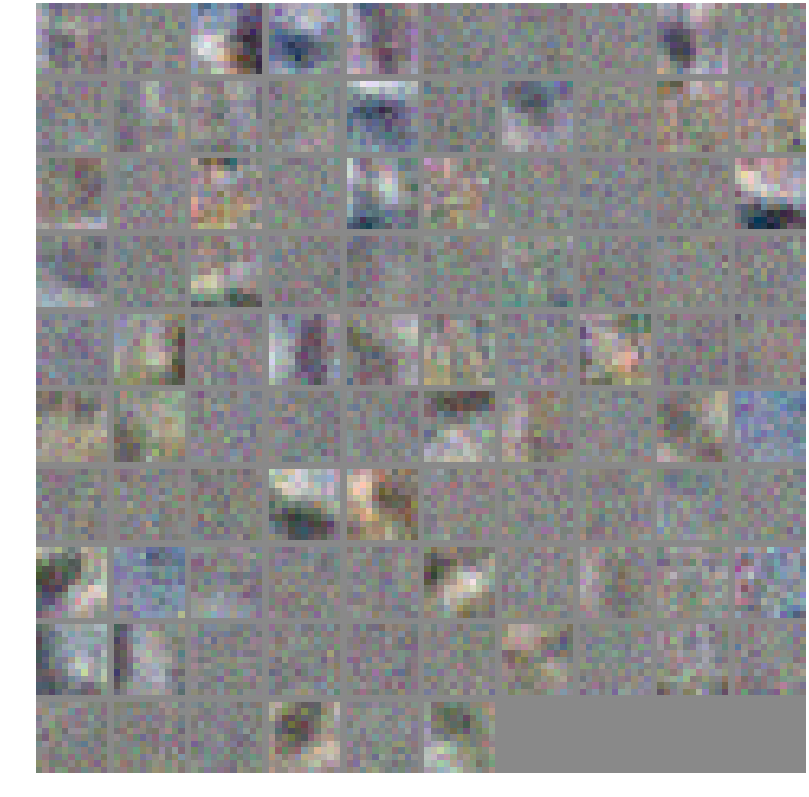
\includegraphics[width=0.49\textwidth]{images/grp0_conv1_weights_color.png}
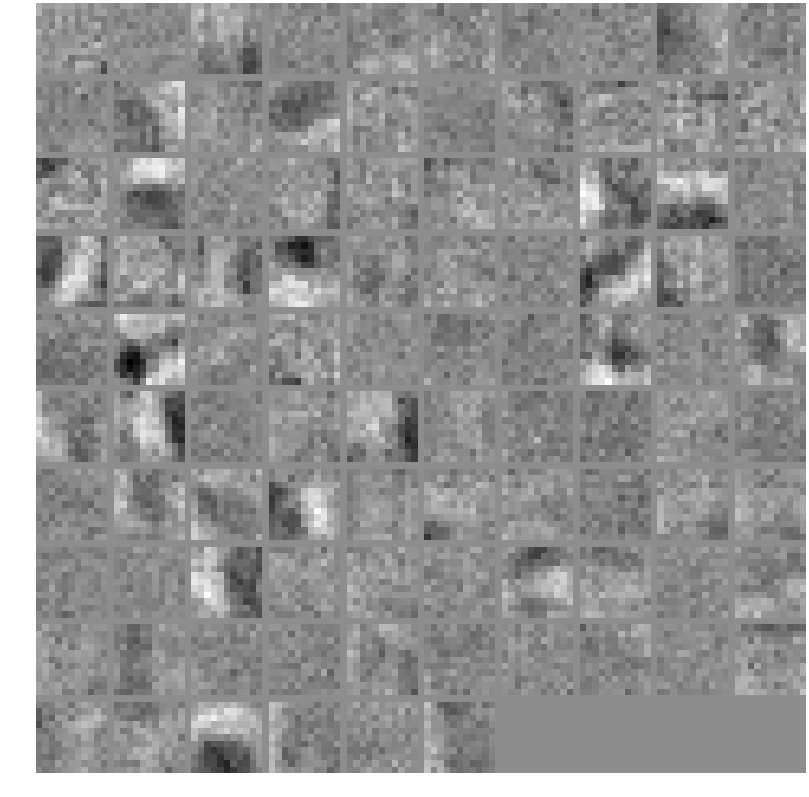
\includegraphics[width=0.49\textwidth]{images/grp0_conv1_weights_gray.png}
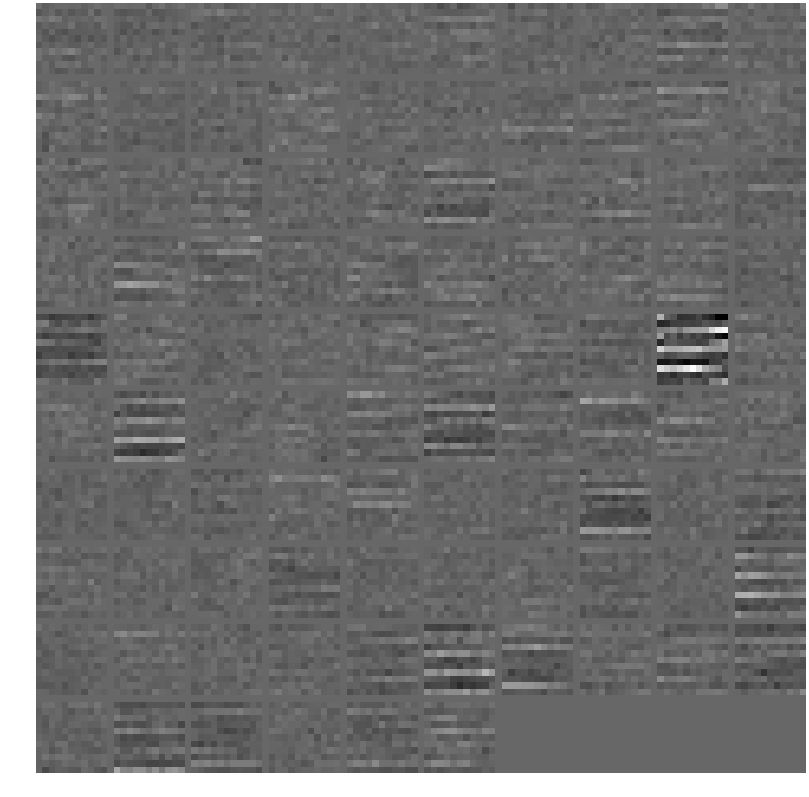
\includegraphics[width=0.49\textwidth]{images/grp0_conv1_weights_lid.png}
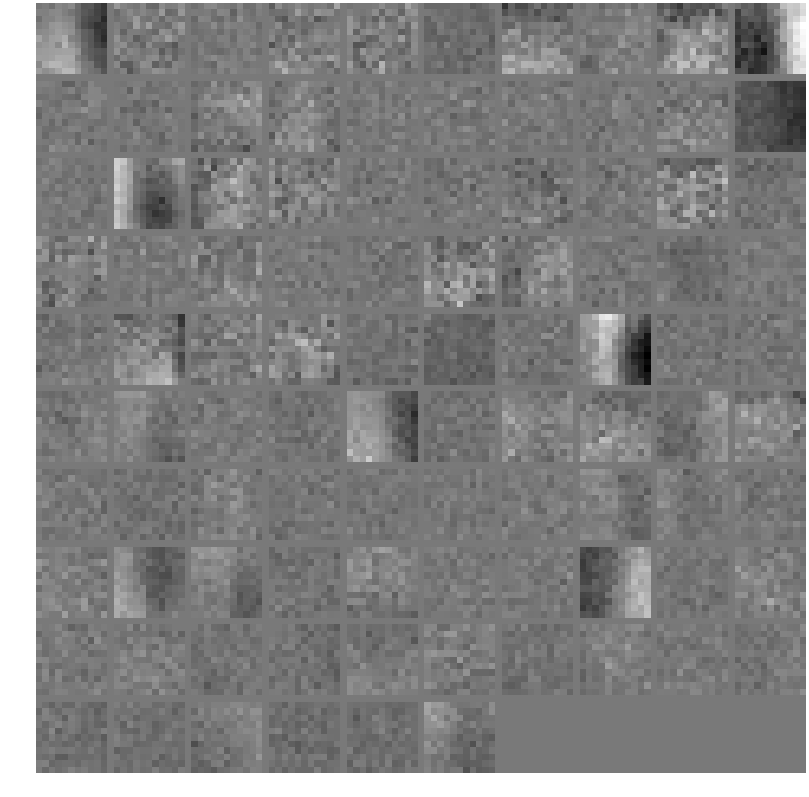
\includegraphics[width=0.49\textwidth]{images/grp0_conv1_weights_lid_depth.png}
\caption{Weights of the first convolutional layer of different feature maps, from top-left to bottom-right: color, grayscale, lidar and interpolated lidar}
\label{fig:filters}
\end{figure}

With the several millions of parameters contained in a neural network, this is not a particularly easy task. However several methods have been developed to visualize neural networks. The simplest and remarkably effective way to investigate the strength of the learning is to look at the first-order convolutional layers. The filters in those layers are applied directly on the image and they therefore contain first-level patterns the network learns. The first-order filters that are learned from some of the main individual feature maps are shown in Figure \ref{fig:filters}. Note first that all of the maps, except the images from the color camera, do only have one layer and are therefore shown in grayscale. 

It is immediately clear that several general filters are learned, but the filters are not all strong and some are relatively noisy. Focusing on the filters from the color images, it is clear that those color images do not really add significant information compared to the grayscale versions, as there are barely color filters and instead mostly structural filters in several color variations. Only one blue filter is present, which appears to trigger on the sky. On the lidar filters the strength of the interpolation preprocessing is apparent, the non-interpolated version has only some noisy ribbed filters, showing the apparent complexity of handling the preprocessing with the network. For all networks it is however clear that a more than half of the filters are considered 'dead' as they only contain a noise pattern. Thus only some edge and corner filters are learned, suggesting that a limited number of filters is apparently adequate for solving the task.
%Approximately half of the filters can however be considered 'dead' as they contain only a noise pattern, from which it appears only a limited number of filters is apparently adequate for solving the task.

\begin{figure}[t]
\centering
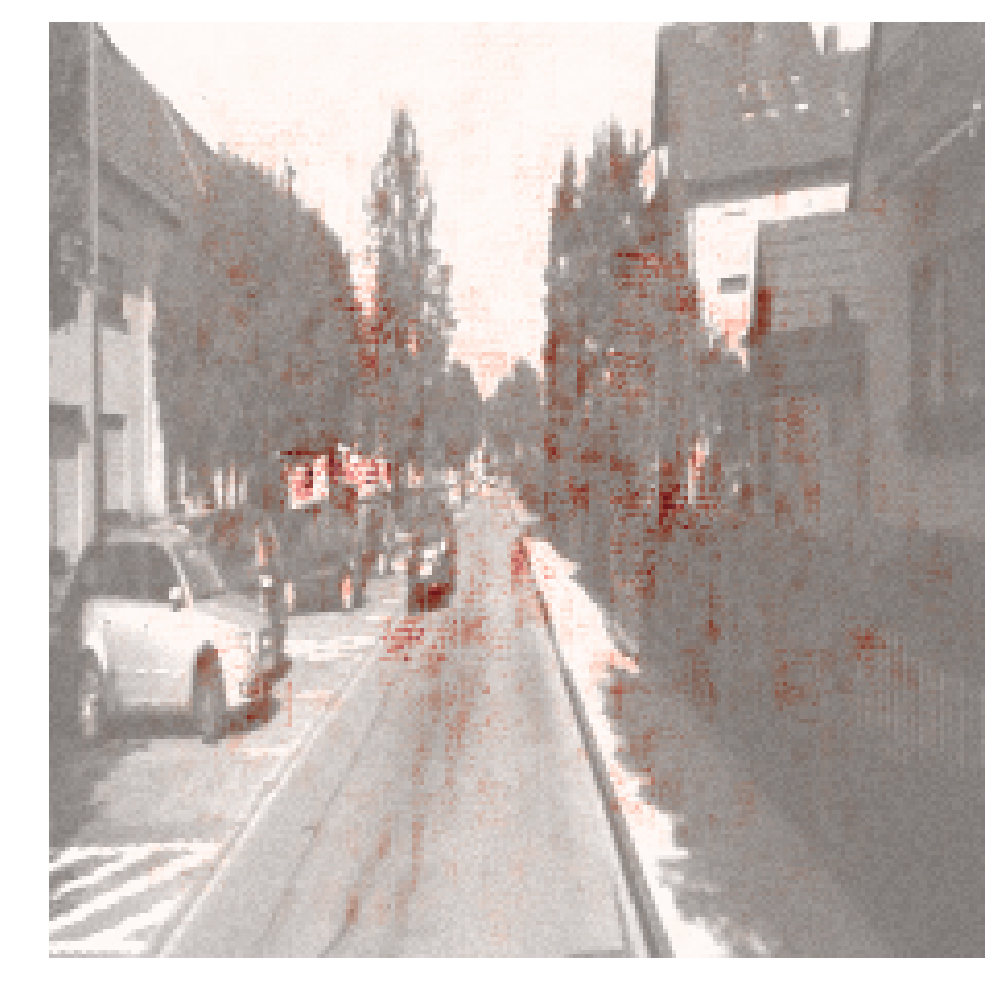
\includegraphics[width=0.49\textwidth]{images/saliency_1-0.png}
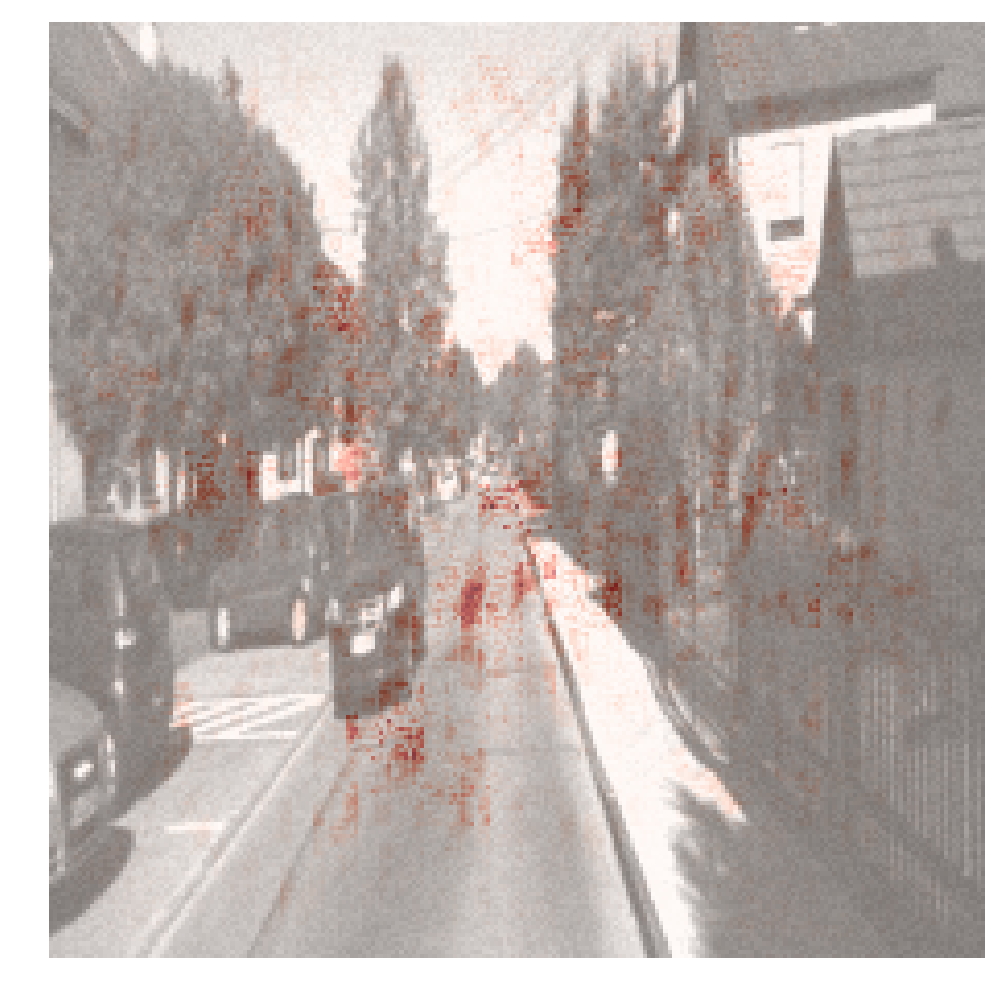
\includegraphics[width=0.49\textwidth]{images/saliency_1-1.png}
\caption{Saliency maps on the grayscale feature maps of two frames in the sequence shown in Figure \ref{fig:frames}, the darker the red colour the stronger the pixel influences the output permutation}
\label{fig:saliency}
\end{figure}

To investigate in more detail where the network focuses on, an alternative visualizing technique is investigated: saliency maps. Figure \ref{fig:saliency} shows saliency maps on the grayscale feature map in two frames. The saliency map should give an indication of the most important part of the image in the classification. Unfortunately it does not show particular attention to a certain detail of a particular kind of object, for example cars. There is also not an very apparent overlap between the same objects tracked through multiple frames in the sequence. Instead the most important part of the image appear to be focused on the part further away in every single frame, suggesting that a zoomed in version might be used to compare the frames directly. Interestingly enough it appears that the network is partly ignoring the moving car, just focusing on the parts which remain static in both images.  

Directly correlating corresponding parts in the image would be an anticipated approach, but it has not been expected to be so efficient, given the complex movement around the streets, with cars passing in the other direction, traffic crossing the street and the car turning in turns, but this picture seems to indicate that the indirect correlation approach comparing the relatively simple patterns learned from the backbone network between the different images might still be a strong approach. It is however hard to conclude this confidently, as the saliency maps do not necessarily give the complete picture. Moreover, this technique has not been applied in this context before and there exists therefore no relevant literature to verify the applicability of this approach in this context.

%A similar approach to find the important regions on the image is to find the location of the maximal activated neurons in the higher layers, for example in the fifth convolutional layer. For comparison with the previous approach the 5 maximal regions are shown for one of the frames investigated with the saliency map is shown in Figure \needfig. It is again hard to point which features the network is exactly focusing on, but there seems again a general tendency on several general static objects, for example trees around and the contour in the road. It remains however difficult to generalize a particular feature over multiple frames.
